\documentclass{article}

\usepackage{color}
\usepackage[usenames,dvipsnames,svgnames,table]{xcolor}
\usepackage{graphicx} 
\usepackage{listings} 
\usepackage{textcomp} 

\newenvironment{componentoption}[2]%
{\textbf{#1}\newline}

\newcommand{\aliases}[1] {\newline \textit{Aliases - } #1}
\newcommand{\defaultvalue}[1] {\newline \textit{Default Value - } #1}
\newcommand{\valuetype}[1] {\newline \textit{Value Type - } \textbf{#1}}


\begin{document}
\raggedright

\definecolor{listinggray}{gray}{0.9}
\definecolor{lbcolor}{rgb}{0.95,0.95,0.95}
\lstset{
backgroundcolor=\color[rgb]{0.95,0.95,0.95},
    tabsize=4,
    language=[GNU]C++,
        basicstyle=\scriptsize,
        upquote=true,
        aboveskip={1.5\baselineskip},
        columns=fixed,
        showstringspaces=false,
        extendedchars=false,
        breaklines=true,
        prebreak = \raisebox{0ex}[0ex][0ex]{\ensuremath{\hookleftarrow}},
        frame=single,
        showtabs=false,
        showspaces=false,
        showstringspaces=false,
        identifierstyle=\ttfamily,
        keywordstyle=\color{Blue},
        commentstyle=\color{DarkGreen},
        stringstyle=\color[rgb]{0.627,0.126,0.941},
        numberstyle=\color[rgb]{0.205, 0.142, 0.73}
}

  


\title{MultiThreading Plugin}
\author{Federico Spadoni\\[\baselineskip]federico.spadoni@inria.fr}

\maketitle

\begin{abstract}

The multithreading plugin has been developed to parallelize computationally intensive tasks without modifiyng the architecture of SOFA and it was highly inspired by Nulstein open source project.\footnote{http://software.intel.com/en-us/articles/do-it-yourself-game-task-scheduling}
To exploit the CPU parallelism it uses the task and scheduler design.
That is an efficient way to scale the computation to all the CPU cores available on
a machine without directly manipulating threads.


\end{abstract}



\section{Requirements}

SOFA Packages:
The following entry must be enabled in CMake.
\begin{itemize}
\item SOFA-PLUGIN\_MULTITHREADING
\end{itemize}

External Libraries:
\begin{itemize}
\item Boost - version 1.50 or later
\end{itemize}

SOFA Plugins:
The following must be loaded in your SOFA instance
\begin{itemize}
\item MultiThreading
\end{itemize}


\section{Tasks and Scheduler Overview}

In task based parallelism, the computation work load must be functionally decompose into tasks.
A task must be considered as a block of code that executes a fraction of the
work independently to other tasks and can run concurrently.
A task is much lighter in weight  than a thread for the operating system because it doesn't allocate all the resources that a thread needs when it is created.
A task can itself create new tasks.

\begin{figure}[!h]
	\centering
	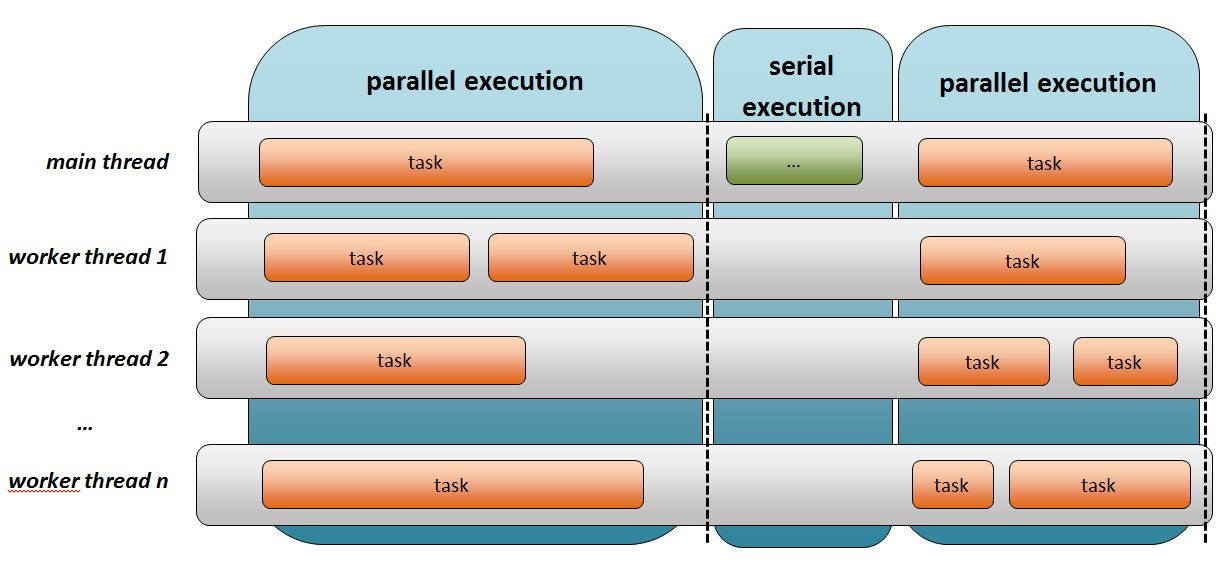
\includegraphics[width=1.0\textwidth]{images/TaskSchedulerDesign.jpg}
	\caption{threads and task distribution}
	\label{fig:multithreading}
\end{figure}


It's important to ensure that all tasks executed concurrently do not have data dependencies between them.
On a multi-core processor it’s possible to execute as many tasks simultaneously as the number of CPU cores.
Systems with hyperthreading technology introduce the concept of logical processors and they can potentially execute two tasks per each physical CPU core.
Some tests with this plugin showed however that for floating point intensive computation there are no advantages from hyperthreading technology in Sofa.\\[\baselineskip]



The scheduler manages the thread pool and assigns tasks to threads.
To avoid the over-subscription of threads the scheduler creates one worker thread for each CPU, takes care of the threads synchronization and tries to balance the work load of each thread, mapping the task execution to fit available worker threads.\\[\baselineskip]

A worker thread keeps its own queue of tasks to execute and can work independently from other threads.
When a queue of a worker thread becomes empty the scheduler tries to steal some tasks from the end of a not empty queue of another worker thread.
When there are no more tasks to execute or to steal the thread goes idle and waits for new tasks.



\section{Task and Scheduler Interfaces}

The main classes the plugin provides are the task scheduler and the task base class interface.

\subsection{Task Scheduler}

The $TaskScheduler$ is a singleton global class that is instantiated the first time it is called and destroyed when Sofa GUI is shut down.
The scheduler must be only initialized calling the start function and passing the $num\_threads$ to create it. 
Task Scheduler uses the $boost::thread$ library to manage the threads.
During the initialization $num\_threads$ worker threads are created and are idle to consume no CPU time.


\begin{lstlisting}

	TaskScheduler::getInstance().start( num_threads );
	
\end{lstlisting}

If the $num\_threads$ parameter is not specified the scheduler creates $N-1$ worker threads on a computer with $N$ cores. 


\subsection{Tasks Implementation}

To implement a task, a class inheriting from $Task$ base class must be defined and the pure virtual function $run$ must be overridden.
After a task is added in the queue there is no control of which thread it will execute.
It's manadatory to pass a pointer to a $Task::Status$ to the class constructor. 
The $Task::Status$ class is a flag that can be used to query if the task completed the execution or if it is still running.
To better understand how to create tasks from Sofa code it is useful to look at the code of the components already implemented in the plugin.

\begin{lstlisting}

#include "Task.h"

class MyTask : public Task
{
public:

	MyTask( Task::Status* status )
		: Task(status) 
		{}
		

	virtual bool run(WorkerThread* )
	{
	// do something
	}

};

\end{lstlisting}



\subsection{Tasks Creation and Queuing}

The tasks must be allocated at run-time and they are added in the current worker thread queue by passing a pointer to the $addTask()$ function. 
The $addTask()$ function is not a blocking function and the current thread keeps executing the code, and it can create and queue other tasks.
The destruction of a task is implicit.


\begin{lstlisting}
{
	Task::Status status;

	MyTask* task = new MyTask( &status );

	WorkerThread* curThread = WorkerThread::getCurrent();

	curThread->addTask( MyTask );

	..
	..

}
\end{lstlisting}


\subsection{Tasks Syncronization}
The function $workUntilDone()$ must be called to wait until all the tasks with the same status flag are executed.
This is a blocking function but the current thread won't be idle.
It will stop executing the succeeding code and start to execute tasks in the queue.

\begin{lstlisting}
{
	Task::Status status;

	MyTask* task = new MyTask( &status );

	WorkerThread* curThread = WorkerThread::getCurrent();

	curThread->addTask( MyTask );

	curThread->workUntilDone(&status);
}
\end{lstlisting}


Other ways to syncronize tasks is to query the $Task::Status$ flag.


\begin{lstlisting}
{
	Task::Status status;

	MyTask* task = new MyTask(&status);

	WorkerThread* curThread = WorkerThread::getCurrent();

	curThread->addTask( MyTask );

	while ( status.IsBusy() )
	{
		// do something while tasks with 
		// the same status flag complete
	}

}
\end{lstlisting}

\begin{lstlisting}
{
	Task::Status status;

	while(;;)
	{
		if ( !status.IsBusy() )
		{
		
			MyTask* task = new MyTask(&status);

			WorkerThread* curThread = WorkerThread::getCurrent();

			curThread->addTask( MyTask );
		}
		
		// do something
		
	}

}
\end{lstlisting}


\section{Components}

These components are included in the plugin and they provide a few examples on how to decompose the work into tasks.

$AnimationLoopParallel$ shows how to create tasks at the component level, running concurrently two or more components of the same type.

$BeamLinearMapping\_mt$ creates tasks to parallelize some floating point computation inside the $for$ loops.

\subsection{AnimationLoopParallel and DataExchange}

The $AnimationLoopParallel$ component was implemented to run the physics simulation of independent scenes concurrently.
The component looks for $BaseAnimationLoop$ components in all its child nodes and executes the $step()$ function of each AnimationLoop concurrently.
The $DataExchange$ component can manage the sharing of data between all the concurrent scenes without being bound by synchronization locks. To avoid the use of synchronization locks, each component in different scenes must have its own copy of the same data to share, and the data synchronization is executed serially.
After the data synchronization the VisualLoop is executed in serial(Fig.~\ref{fig:multithreading}).
Each child node of the node where the AnimationLoopParallel is placed must be seen as a independent scene and there should be no physics interaction or collision detection between these scenes.
When all the step functions return, the visual loop (graphics rendering) is executed serially throughout the scene.

\begin{figure}[!h]
	\centering
	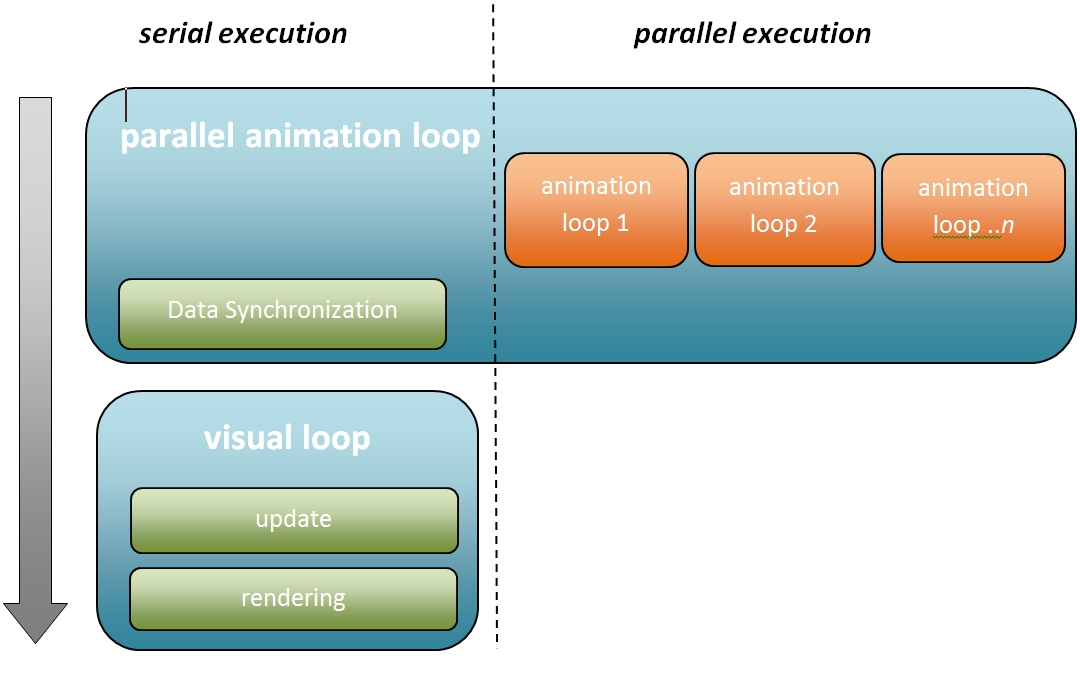
\includegraphics[width=1.0\textwidth]{images/multithreading.jpg}
	\caption{simulation loop: serial and parallel code}
	\label{fig:multithreading}
\end{figure}


The DataExchange component must be placed in the same node where the AnimationLoopParallel is and the path links to the source and destination data to copy must be defined.
The data template of the source and destination path links must be the same.
This data synchronization is executed serially before the VisualLoop is executed.
A common use of the AnimationLoopParallelScheduler component is to place it in the root node of the scene hierarchy and add a AnimationLoop to all the child nodes you want to be executed independently.

Below is detailed the AnimationloopParallel $step()$ function implementation. 
A $boost::pool<>$ is used for fast task allocation:


\begin{lstlisting}
void AnimationLoopParallel::step(const core::ExecParams* params, double dt)
{

	static boost::pool<> task_pool(sizeof(StepTask));

	if (dt == 0)
		dt = this->gnode->getDt();


	Task::Status status;

	WorkerThread* thread = WorkerThread::getCurrent();	



	typedef Node::Sequence<simulation::Node,true>::iterator ChildIterator;
	for (ChildIterator it = gnode->child.begin(), itend = gnode->child.end(); it != itend; ++it)
	{
		if ( core::behavior::BaseAnimationLoop* aloop = (*it)->getAnimationLoop() )
		{
			thread->addTask( new( task_pool.malloc()) StepTask( aloop, dt, &status ) );

		}

	}

	thread->workUntilDone(&status);



	double startTime = gnode->getTime();
	gnode->setTime ( startTime + dt );

	// exchange data event
	DataExchangeEvent ev ( dt );
	PropagateEventVisitor act ( params, &ev );
	gnode->execute ( act );


	// it doesn't call the destructor
	task_pool.purge_memory();
}
\end{lstlisting}
	
	
This is the StepTask definition. All the class members needed to call the AnimationLoop $step()$ function are passed in the constructor:
\begin{lstlisting}
StepTask::StepTask(core::behavior::BaseAnimationLoop* aloop, const double t, Task::Status* status) 
		: Task(status)
		, dt( t )
		, animationloop(aloop)
	{
	}
	
	bool StepTask::run(WorkerThread* )
	{
		animationloop->step( core::ExecParams::defaultInstance() ,dt);
		return true;
	}
\end{lstlisting}



\subsubsection{AnimationLoopParallel tips and limitations}

To get the best performance with the AnimationLoopParallel component, the execution time of each animation loop should be manually balanced to get almost the same time length. 
If in the scene an animation loop is computationally more expensive, the MultiStepAnimationLoop component can be useful not to limit the speed of execution of a potentially faster AnimationLoop step function.
This will improve the synchronization between threads, minimizing the waiting time for all animation loops completion.
The scene should be split into as many independent scenes as possible.
An independent scene is considered as a scene where the physics simulated objects are never supposed to collide with the objects of another scene during the whole simulation time length.\\[\baselineskip]

The main limitation using the AnimationLoopParallel is that interaction with the mouse with the objects in the scene crashes the simulation.\\[\baselineskip]


\subsubsection{AnimationLoopParallel attributes}

\begin{componentoption}{threadNumber}

The number of threads the scheduler must create. 
If that value is 0 the scheduler creates $N-1$ worker threads on a computer with $N$ physical cores (hyperthreading ignored). 
\valuetype{int}
\defaultvalue{0}
\end{componentoption}


\subsubsection{DataExchange attributes}

\begin{componentoption}{template}

The defined template type must match the data type in both the $from$ and $to$ attribute values. Common \textit{Value Type: }
\begin{itemize}
  \item bool
  \item double
  \item float
  \item Vec3f 
  \item Vec3d
  \item vector$<$float$>$
  \item vector$<$double$>$
  \item vector$<$int$>$
  \item vector$<$unsigned\_int$>$
  \item vector$<$Vec3f$>$ 
  \item vector$<$Vec3d$>$
  \item vector$<$Vec2f$>$
  \item vector$<$Vec2d$>$
\end{itemize}
If a data type is missing it can be added in the DataExchange.cpp file.
The template class of the data type to add must be instantiated and then added to the factory class using the RegisterObject $add()$ function.

\begin{lstlisting}
template class SOFA_MULTITHREADING_PLUGIN_API DataExchange< MyType >;

int DataExchangeClass = core::RegisterObject("DataExchange")
.add< DataExchange< MyType > >
\end{lstlisting}

\end{componentoption}


\begin{componentoption}{from}

Defines the path to the destination location in the scene of the data you want to copy. The path must start with the @ symbol
\end{componentoption}


\begin{componentoption}{to}

Defines the path to the source location in the scene of the data you want to copy. The path must start with the @ symbol.\\[\baselineskip]
\end{componentoption}



\subsubsection{Example file scenes}

applications/plugins/MultiThreading/scenes/TriangularForceFieldComparison.scn

applications/plugins/MultiThreading/scenes/Livers.scn



\subsection{BeamLinearMapping\_mt}

This component inherits all the functionality from the $BeamLinearMapping$ component and overrides three virtual functions that contain a $for$ loop: $apply()$, $applyJ()$ and $applyJT()$.
It adds only one data attribute, the $granularity$. This attribute sets the number of iterations of the $for$ loop, corresponding to the number of points along the beam elements that must be assigned and executed for each task. If this number is lower than the number of iterations the loop won't be parallelized and the corresponding $BeamLinearMapping$ function is called.  If this number is greater than the number of iterations of the loop the tasks are created and each task executes the $granularity$ value of iterations of the loop.

In the initialization the scheduler is instantiated with a default number of worker threads.

task definition:
\begin{lstlisting}

class applyTask : public simulation::Task
{
	
	typedef typename BeamLinearMapping<TIn,TOut>::Out::VecCoord  VecCoord;
	typedef typename BeamLinearMapping<TIn,TOut>::In::VecCoord  InVecCoord;

public:

	virtual bool run( simulation::WorkerThread* );

protected:

	applyTask( const simulation::Task::Status* status );

private:

	BeamLinearMapping_mt<TIn,TOut>* _mapping;
		
	const helper::ReadAccessor< Data< typename In::VecCoord > >* _in;
	helper::WriteAccessor< Data< typename Out::VecCoord > >* _out;

	unsigned int _firstPoint;
	unsigned int _lastPoint;

	friend class BeamLinearMapping_mt<TIn,TOut>;
};
	
// run function definition
template <class TIn, class TOut>
bool BeamLinearMapping_mt< TIn, TOut>::applyTask::run( simulation::WorkerThread* )
{
	bool result = true;

	for(int i = _firstPoint; i < _lastPoint; ++i )	
	{
		Coord inpos = _mapping->points[i];
		int in0 = helper::rfloor(inpos[0]);
		if (in0<0) 
			in0 = 0; 
		else if (in0 > (int)_in->size()-2) 
			in0 = _in->size()-2;
		inpos[0] -= in0;

		const In::Coord _in0 = (*_in)[in0];
		const In::Coord _in1 = (*_in)[in0+1];
		Real beamLengh = _mapping->beamLength[in0];
		Coord& rotatedPoint0 = _mapping->rotatedPoints0[i];
		Coord& rotatedPoint1 = _mapping->rotatedPoints1[i];

		rotatedPoint0 = _in0.getOrientation().rotate(inpos) * beamLengh;
		Coord out0 = _in0.getCenter() + rotatedPoint0;
		Coord inpos1 = inpos; inpos1[0] -= 1;
		rotatedPoint1 = _in1.getOrientation().rotate(inpos1) * beamLengh;
		Coord out1 = _in1.getCenter() + rotatedPoint1;
			
		Real fact = (Real)inpos[0];
		fact = 3*(fact*fact)-2*(fact*fact*fact);
		(*_out)[i] = out0 * (1-fact) + out1 * (fact);

	}

	return result;
}
\end{lstlisting}


The following code is the $apply()$ function, one of the overriden function from the $BeamLinearMapping_mt$ component.
Inside all these overriden functions there is an optimization to prevent the $false$ $sharing$ data problem.\footnote{http://software.intel.com/en-us/articles/false-sharing} As a rule of thumb the distance of memory address read and written from different cores must be separated by at least one cache line (64 bytes on most of the computer) to prevent cache missing of the data. This was straightforward to prevent due to the beam chain structure, but it is not an easy problem to deal whit in the general case.


\begin{lstlisting}
template <class TIn, class TOut>
	void BeamLinearMapping_mt< TIn, TOut>::apply(const core::MechanicalParams* mparams /* PARAMS FIRST */, Data<VecCoord>& _out, const Data<InVecCoord>& _in)
{

	static boost::pool<> task_pool(sizeof(BeamLinearMapping_mt< TIn, TOut>::applyTask));

	unsigned int numPoints = points.size();

	if ( numPoints >  2*mGrainSize.getValue()  )
	{		
		helper::WriteAccessor< Data< typename Out::VecCoord > > out = _out;
		helper::ReadAccessor< Data< typename In::VecCoord > > in = _in;

		rotatedPoints0.resize(points.size());
		rotatedPoints1.resize(points.size());
		out.resize(points.size());


		// create tasks
		simulation::Task::Status status;
		simulation::WorkerThread* thread = simulation::WorkerThread::getCurrent();	

		//const int nbThread = simulation::TaskScheduler::getInstance().size();

		// to prevent false sharing it runs the first half of the taskSize
		const int taskSize = 2*mGrainSize.getValue();

		int nbTasks = numPoints / taskSize;
		int pointsLeft = numPoints % taskSize;

		for ( int i=0; i<nbTasks; ++i)
		{
			BeamLinearMapping_mt< TIn, TOut>::applyTask* task = 
					new( task_pool.malloc()) BeamLinearMapping_mt< TIn, TOut>::applyTask( &status );

			// task private members are set
			task->_mapping = this;
			task->_in = &in;
			task->_out = &out;
			task->_firstPoint = i*taskSize;
			task->_lastPoint = i*taskSize + mGrainSize.getValue();

			thread->addTask( task );

		}
		if ( pointsLeft > 0)
		{
			BeamLinearMapping_mt< TIn, TOut>::applyTask* task = 
					new( task_pool.malloc()) BeamLinearMapping_mt< TIn, TOut>::applyTask( &status );

			// task private members are set
			task->_mapping = this;
			task->_in = &in;
			task->_out = &out;
			task->_firstPoint = nbTasks*taskSize;
			task->_lastPoint = nbTasks*taskSize + pointsLeft;

			thread->addTask( task );

		}
		// wait all tasks with the same status complete
		thread->workUntilDone(&status);


		// it runs the second half of the taskSize
		for ( int i=0; i<nbTasks; ++i)
		{
			BeamLinearMapping_mt< TIn, TOut>::applyTask* task = 
					new( task_pool.malloc()) BeamLinearMapping_mt< TIn, TOut>::applyTask( &status );

			// task private members are set
			task->_mapping = this;
			task->_in = &in;
			task->_out = &out;
			task->_firstPoint = i*taskSize + mGrainSize.getValue();
			task->_lastPoint = i*taskSize + taskSize;

			thread->addTask( task );

		}

		// wait all tasks with the same status complete
		thread->workUntilDone(&status);

	}
	else
	{

		BeamLinearMapping<TIn,TOut>::apply( mparams, _out, _in );

	}

	// it doesn't call the destructor
	task_pool.purge_memory();

}

	
\end{lstlisting}


\subsubsection{BeamLinearMapping\_mt tips}

The $granularity$ is helpful to amortize task scheduling overhead time. 

In the general case there is not an exact value and some tests must be done the choose it. Comparing the speed (fps) of the simulation while running the scene with different granularity can help to choose a resonable value.

In some specific cases, if the number of cores in the processor and the number of iterations of the loops inside the overridden functions are known, this value can be optimized to distribute the work load evenly and limit the task scheduling overhead time. For instance, with a 100 iterations loop in a 2 core processor the granularity can be set at 50. Two tasks will be created and they both will execute 50 iterations. (taking into account the specific $BeamLinearMapping\_mt$ optimization, a good value is 25). 



\subsubsection{BeamLinearMappingParallel attributes}

%BeamLinearMapping_mt% inherits all the attributes from the %BeamLinearMapping% component and defines only the granularity.\\[\baselineskip]


\begin{componentoption}{granularity}

This attribute sets the maximum number of points along the beam structure that must be processed for each task.
\valuetype{unsigned int}
\defaultvalue{32}
\end{componentoption}



\subsubsection{Example file scenes}


applications/plugins/MultiThreading/scenes/BeamLinearMapping\_mt.scn\\[\baselineskip]




\subsection{BeamFemForceFieldParallel}

to be done


\end{document}
